\documentclass[final]{beamer} % use beamer

%\usepackage[usenames,dvipsnames]{xcolor}
\usepackage[orientation=landscale,size=a0,scale=1.6]{beamerposter}
\usepackage[english]{babel}
\usepackage[utf8]{inputenc}
\usepackage{amsfonts}
\usepackage{amsthm}
\usepackage{amsmath}
\usepackage{pgf}
\usepackage{palatino}
\usepackage{natbib}
\usepackage{paralist}
\usepackage{epstopdf}
\usepackage{algorithm}
\usepackage{caption}
\usepackage{algorithmic}
\setbeamertemplate{bibliography item}[text]

\setlength{\leftmargini}{2cm}


%\usetheme{bpiresicml2013}
\usepackage{beamerthemebpiresicml2013}

%\setbeamercolor{block title}{fg=black,bg=white}
%\setbeamercolor{block body}{fg=black,bg=white}
%--set colors for alerted blocks (with frame)----------------------------------
%--textcolor = fg, backgroundcolor = bg, dblue is the jacobs blue
%\setbeamercolor{block alerted title}{fg=white,bg=uofagreen!70}%frame color
 %\setbeamercolor{block alerted body}{fg=black,bg=uofagreen!10}%body color

%==Title, date and authors of the poster=======================================

\newcommand{\eps}{\epsilon}
\DeclareMathOperator{\pol}{Poly}
\newcommand{\poly}[1]{\pol\left(#1\right)}
\newcommand{\EEp}[1]{\mathbb{E}\left[#1\right]}
\newtheorem{thm}{Theorem}[section]

%\addtobeamertemplate{block begin}{}{\setlength{\parskip}{35pt plus 1pt minus 1pt}}

\title{Deterministic Independent Component Analysis }
\author{Ruitong Huang, Andr\'as Gy\"orgy, Csaba Szepesv\'{a}ri}


\begin{document}

\begin{frame}[c]
	\vspace{-1.5cm}

	\begin{columns}[t,totalwidth=\textwidth]
	
	\begin{column}{0.01\textwidth}
	\end{column}
%------------------------------------------------------------------------------
% The first column
%------------------------------------------------------------------------------	

 	\begin{column}{.24\textwidth}% the right size for a 3-column layout
		\begin{block}{Indep. Component Analysis (ICA)}
		\vspace{-1.5cm}
			\begin{equation*}
			\label{eq:stoch-ICA}
			X = AS+\epsilon
			\end{equation*}
			\vspace{1cm}
			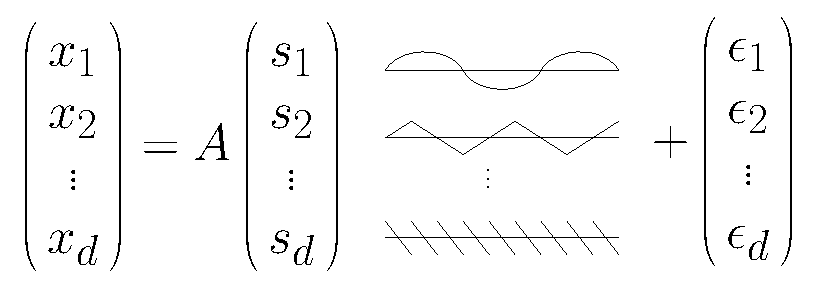
\includegraphics[width=0.9\textwidth]{ICA_model.eps}
			\begin{itemize}
				\item $S = (S_1,\ldots, S_d)$ are non-Gaussian variables, and	$\eps \sim \mathcal{N}(0,\Sigma)$ is a Gaussian noise. 
				\item Goal: Given independent observations $X(1), \ldots, X(T)$, reconstruct $A$ up to scaling and permutation.
				\item Independence? $S_1(t),\ldots, S_d(t)$, $\eps_1(t), \ldots, \eps_d(t)$ are mutually independent for any $t$.
				\item for simplicity, we assume $A$ is non-singular. 
				\item Applications of ICA	
				\begin{itemize}
						\item Blind Source (Signal) Separation;
						\item Medical Imaging.
				\end{itemize}				
			\end{itemize}						
		\end{block}
		\vspace{1.0ex}
	
		\begin{block}{Previous works}
			The literature in ICA is vast in both practical algorithms and theoretical analyses. We only name a few here that are most relavent to our work.
			\begin{itemize}
				\item Fast ICA \citep{hyvarinen1999fast};
				\begin{itemize}
					\item Finite-sample performance only available in the noise-free case.   
				\end{itemize}
				\item Arora et al.'s method \citep{arora2012provable};
				\begin{itemize}
					\item Depends on some unspecified parameter;
				\end{itemize} 
				\item Moment methods;
				\begin{itemize}
					\item Hsu and Kakade's method  \citep{hsu2013learning} (HKICA);
					\item Frourier PCA \citep{goyal2014fourier} (FPCA);
				\end{itemize}
			\end{itemize}
		\end{block}

	\end{column}
%------------------------------------------------------------------------------
% The second column
%------------------------------------------------------------------------------	
	\begin{column}{0.01\textwidth}
	\end{column}
	
	\begin{column}{.24\textwidth}% the right size for a 3-column layout
		\begin{block}{HKICA}
		Normally, moment methods require a tensor decomposition step. We take HKICA as an example.
		\vspace{1cm}
		\begin{figure}
		\centering
		\caption*{The HKICA method}
		\begin{algorithmic}[1]
		\STATE Let $f(\eta) = \EEp{(\eta^{\top}x)^4} - 3 \EEp{(\eta^{\top}x)^2}^2$;
		\STATE  Choose $\phi$ and $\psi$; (How?)
		\STATE Let $T(\phi) = \nabla^2 f(\phi)$. Then 
		\[T(\phi) = AK 
		\left(
		\begin{array}{ccc}
		\sigma_1 & & \\ %\left(\frac{\phi^{\top}A_1}{\psi^{\top}A_1}\right)^2 & &\\
		    & \ddots & \\
		    & & \sigma_d %\left(\frac{\phi^{\top}A_d}{\psi^{\top}A_d}\right)^2\\
		\end{array} 
		\right) 
		A^{\top},
		\]
		where $\sigma_i = \left(\phi^{\top}A_i\right)^2$.
		\STATE Let $M = T(\phi)(T(\psi))^{-1}$. Then 
		\[M = A 
		\left(
		\begin{array}{ccc}
		\lambda_1 & & \\ %\left(\frac{\phi^{\top}A_1}{\psi^{\top}A_1}\right)^2 & &\\
		    & \ddots & \\
		    & & \lambda_d %\left(\frac{\phi^{\top}A_d}{\psi^{\top}A_d}\right)^2\\
		\end{array} 
		\right) 
		A^{-1},
		\]
		where $\lambda_i = \left(\frac{\phi^{\top}A_i}{\psi^{\top}A_i}\right)^2$.
		\STATE Do an eigen-decomposition of $M$ to recover $A$, assuming all $\lambda_i$'s are distinct.
		\end{algorithmic}
		\end{figure}
		\end{block}
		\vspace{1.0ex}
				
		\begin{block}{Difficulty}
		\large {Problem: Minimal gap of the eigenvalues.}
		\vspace{0.5cm}
		\begin{itemize}
		\item Theoretical analysis shows that the performance depends on 
		\[
		\gamma_A = \min_{i\neq j} \left\vert \lambda_i - \lambda_j\right \vert.
		\]
		\vspace{-0.5cm}
		\item $\gamma_A$ is not yet well understood.
		\item FPCA also depends on some unspecified parameter.
		\item  We aim to develop algorithms that 
			\begin{itemize}
				\item have provable performance;
				\item are polynomial in both computational and sample complexity;
				\item Only depend on natural parameters of the problem.
			\end{itemize}
		\end{itemize}
		\end{block}\vspace{0.5ex}
	\vspace{0.5ex}
	\end{column}
	\begin{column}{0.01\textwidth}
	\end{column}
%------------------------------------------------------------------------------
% The third column
%------------------------------------------------------------------------------
	\begin{column} {.24\textwidth}
		\begin{block}{Our method: Deterministic ICA (DICA)}		
		\begin{figure}
				\begin{algorithmic}[1]
				\STATE Sample $\psi$, $\phi_1$, and $\phi_2$ independently from standard normal distribution.
				\STATE Calculate $\nabla^2 f(\psi)$ and $B$ such that $\nabla^2 f(\psi) = BB^{\top}$.
				\STATE Calculate $T(\phi_1) = \nabla^2 f(B^{-\top}\phi_1)$ and $T(\phi_2) = \nabla^2 f(B^{-\top}\phi_2)$.
				\STATE Calculate $M = T(\phi_1)(T(\phi_2))^{-1}$.
				\[
				M = R \left(
				\begin{array}{ccc}
				\tilde{\lambda}_1 & & \\ 
				    & \ddots & \\
				    & & \tilde{\lambda}_d
				\end{array} 
				\right) 
				R^{\top},
				\]
				where $\tilde{\lambda}_i = \left(\frac{\phi_1^{\top}R_i}{\phi_2^{\top}R_i}\right)^2$.
				\STATE Do an eigen-decomposition of $M$ to recover $R$.
				\STATE Return $\hat{A} = BR$ as an estimation of $A$. 
				\end{algorithmic}
				\end{figure}
				Note that $\tilde{\lambda}$ (and its minimal gap) is now independent to $A$, and easier to analyze.
		\end{block}
		\vspace{0.5ex}
			
		\begin{block}{Result}
		DICA estimates the mixing matrix $A$ from $T$ samples of $x$ such that: 
		\begin{itemize}
		\item the computational complexity of the algorithm is $O(d^3 T)$;
		\item given $T$ large enough, with high probability, there exists a permutation $\pi$ and constants $\{c_1,\ldots,c_d\}$, such that for all $1\le k\le d$, 
		\[\| c_k\hat{A}_{\pi(k)} - A_k\|_2 \le O(\frac{1}{\sqrt{T}}).
		\]
		\vspace{-1cm}
		\end{itemize}
		Simulation result is provided in the paper.
		\vspace{-1cm}
		\end{block}
		\vspace{0.5ex}
		
		\begin{block}{Recursive version}
		\begin{itemize}
			\item Based on the idea of Vempala et al. \citep{vempala2014max};
			\item Change the dependence on the minimal gap to the maximal gap, which helps reduce the sample complexity;
			\item See the paper for details.
		\end{itemize}
		\end{block}
	\end{column}
%------------------------------------------------------------------------------
% The fourth column
%------------------------------------------------------------------------------	

	\begin{column}{0.01\textwidth}
	\end{column}
	\begin{column}{0.24\textwidth}
		\begin{block}{Deterministic?}
		\begin{figure}
		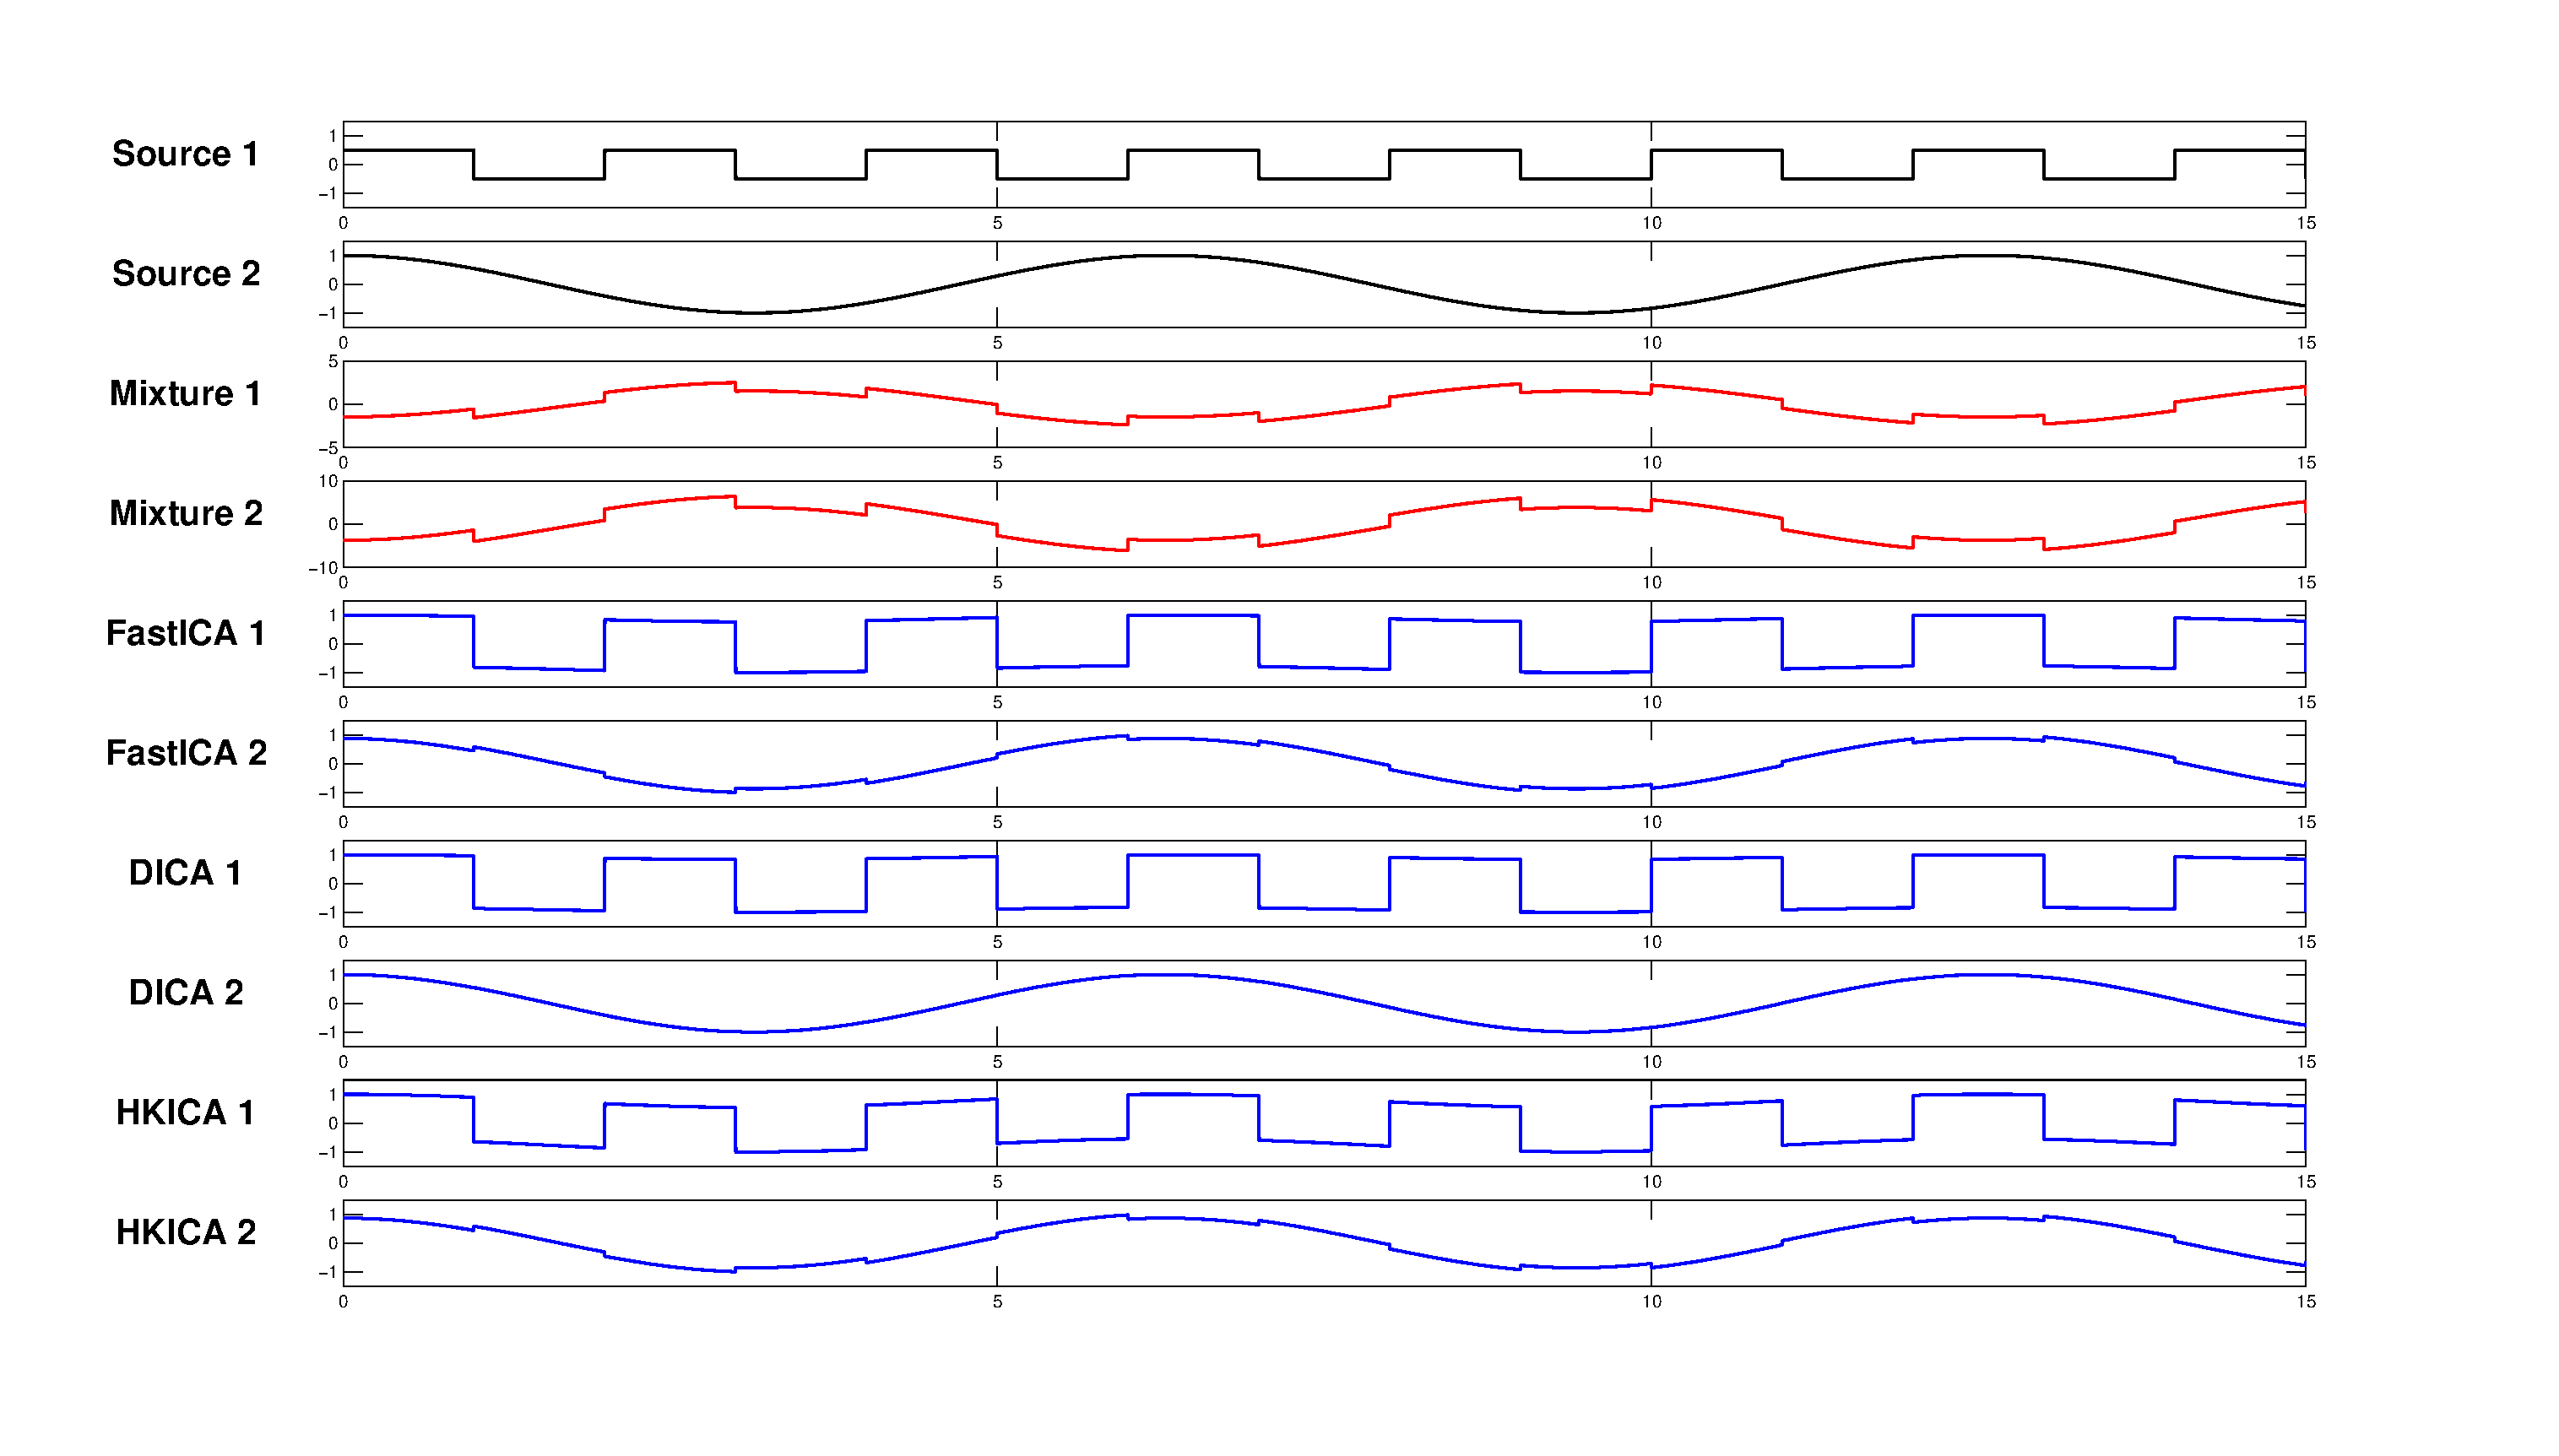
\includegraphics[width = 0.9\textwidth]{demo}
		\caption*{An example of different ICA methods}
		\end{figure} 
		
		\begin{itemize}
		\item It is also known that ICA also works well on unmixing deterministic signals;
		\item All deterministic sequences satisfy the independence assumption;
		\item Could ICA separate any deterministic sequences?
		\end{itemize}
		\begin{center}
		{\large Not really!}
		\end{center}
		We generalize ICA to a non-stochastic setting to cover deterministic signals, and another practically important case, Markov sources.
		
		See the paper for details.
		\end{block}
		\vspace{1ex}

		\begin{block}{References}
		\scriptsize
		\bibliographystyle{plain}
		\bibliography{DICA}
		\end{block}	
		\vspace{1ex}	
		\begin{block}{Acknowledgements}
		\scriptsize
		This work was supported by the Alberta Innovates Technology Futures and NSERC.
		\end{block}
		
	\end{column}
		
	\begin{column}{0.01\textwidth}
	\end{column}
\end{columns}
 
\end{frame}

\end{document}
